\section{Create User Tab}
\subsubsection{Overview}
The \textbf{Create User tab} Allows for the creation of a new user in the server, setting their username, password and role, either being an admin or a user.

\begin{figure}[H]
    \centering
    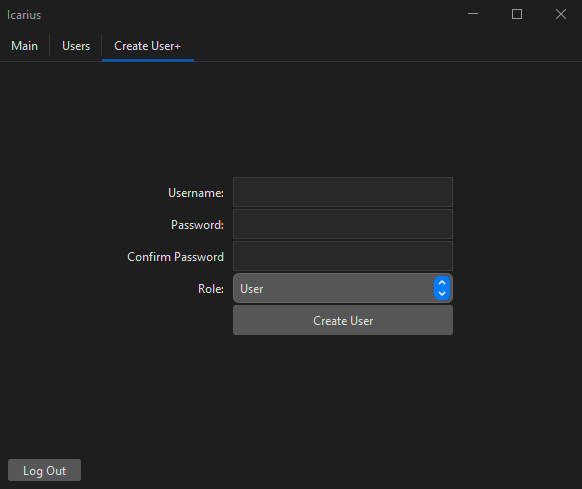
\includegraphics[width=0.6\textwidth]{CreateUserTab/createUserOverview.PNG}
\end{figure}

\subsubsection{Creating a new user}
In order to add a new user, the user must:
\begin{enumerate}
    \item Fill the \textbf{Username}, \textbf{Password} and \textbf{Confirm Password} fields
    \begin{figure}[H]
        \centering
        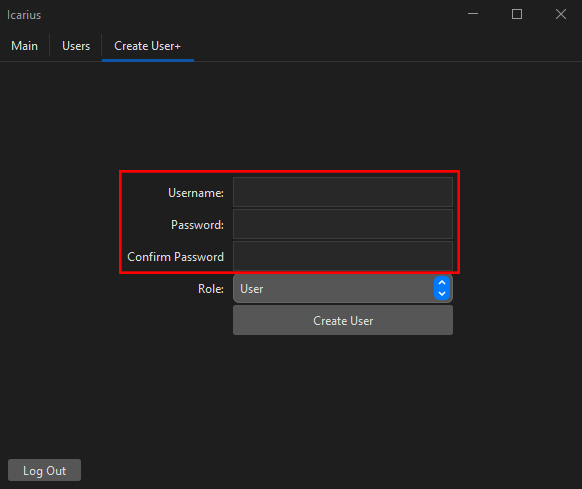
\includegraphics[width=0.6\textwidth]{CreateUserTab/CreateUser/createUserText.PNG}
    \end{figure}

    \item Click on the \textbf{Role} drop-down list to select the new user’s role. This will be either an admin or a user
    \begin{figure}[H]
        \centering
        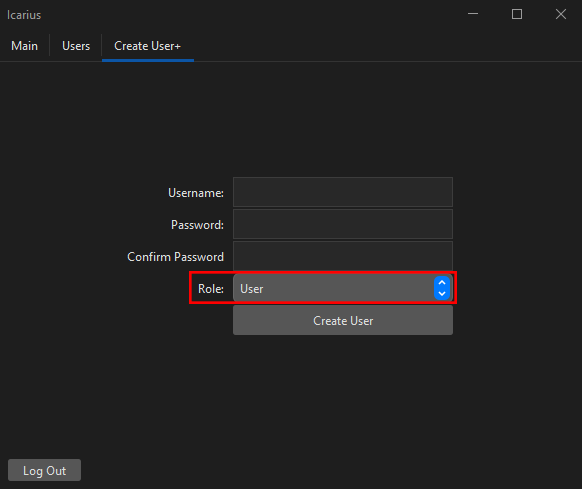
\includegraphics[width=0.6\textwidth]{CreateUserTab/CreateUser/createUserRole.PNG}
        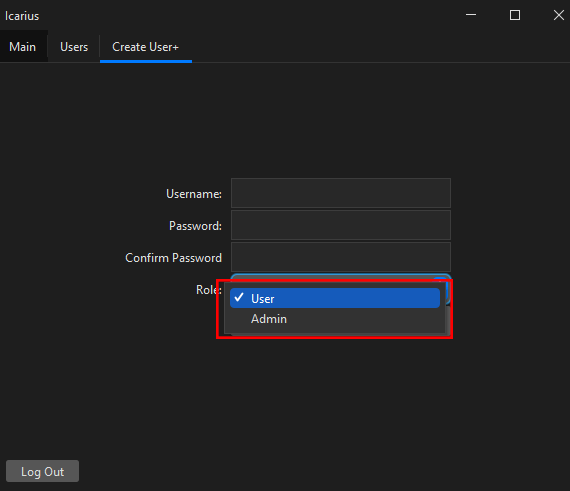
\includegraphics[width=0.6\textwidth]{CreateUserTab/CreateUser/createUserRoleView.PNG}
    \end{figure}

    \item Click on \textbf{Create User}. \textit{This will add the user to the database}
    \begin{figure}[H]
        \centering
        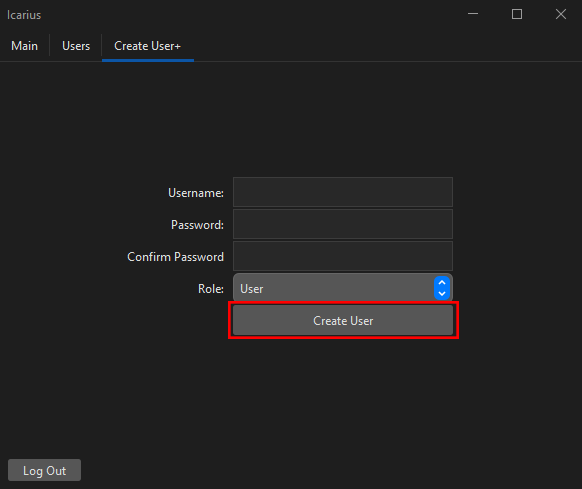
\includegraphics[width=0.6\textwidth]{CreateUserTab/CreateUser/createUserCreate.PNG}
    \end{figure}
\end{enumerate}